% Part: sets-functions-relations
% Chapter: relations
% Section: graphs

\documentclass[../../../include/open-logic-section]{subfiles}

\begin{document}

\olfileid[tr]{sfr}{rel}{grp}
\olsection{Çizgeler}

Bir \emph{çizge}, ``düğüm'' ya da ``köşe'' denilen noktaların kenarlarla
birbirine bağlandığı bir şemadır. Çizgeler, ayrık matematikte ve bilgisayar
biliminde her yerde karşımıza çıkan araçlardır. Çeşitli türden ağlar gibi somut
şeylerden kararların mümkün sonuçları gibi soyut yapılara kadar uzanan bağıntı
ve yapıları temsil etmek ve görselleştirmek için son derece yararlıdırlar.
Literatürde; kenarların yönlü olup olmamasına, etiket taşıyıp taşımamasına, bir
düğümden yine aynı düğüme uzanan kenarlara veya aynı düğümler arasında birden
fazla kenara izin verilip verilmemesine vb. göre farklılaşan pek çok çizge türü
vardır. \emph{Yönlü çizgelerin} bağıntılarla özel bir bağlantısı vardır.

\begin{defn}[Yönlü çizge]
Bir \emph{yönlü çizge} $G=\tuple{V,E}$, bir \emph{köşe kümesi}~$V$ ile bir
\emph{kenar kümesi}~$E \subseteq V^2$'den oluşur.
\end{defn}

\begin{explain}
Tanımımıza göre bir çizge, bir küme ile o küme üzerindeki bir bağıntıdan
ibarettir. Elbette çizgelerden söz ederken onları çizimle temsil etmeyi beklemek
doğaldır: ancak ve ancak $\tuple{v_1,v_2}\in E$ ise $v_1$'den $v_2$'ye bir ok
çizerek bir çizge oluşturabiliriz. Tek başına bir bağıntıyla bir
çizge arasındaki tek fark, çizgenin köşe kümesini ayrıca belirtmesidir; yani
bir çizgenin yalıtılmış köşeleri olabilir. Ancak önemli nokta şudur: bir $X$
kümesi üzerindeki her $R$ bağıntısı $\tuple{X,R}$ yönlü çizgesi olarak
görülebilir; tersine $\tuple{V,E}$ yönlü çizgesi de $V$ kümesi açıkça
belirtilmiş olan bir $E \subseteq V^2$ bağıntısı olarak görülebilir.
\end{explain}

\begin{ex}
$V=\{1,2,3,4\}$ ve
$E=\{\tuple{1,1}, \allowbreak \tuple{1, 2}, \allowbreak \tuple{1, 3},
\allowbreak \tuple{2, 3}\}$ olan $\tuple{V,E}$ çizgesi şöyle görünür:
\begin{align*}
& 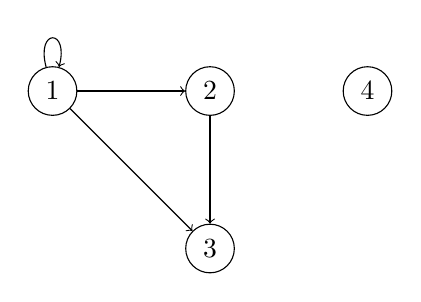
\begin{tikzpicture}[->,node distance=2cm]
  \node[draw,circle] (A) {$1$};
  \node[draw,circle] (B) [right of=A] {$2$};
  \node[draw,circle] (C) [below of=B] {$3$};
  \node[draw,circle] (D) [right of=B] {$4$};
  \draw (A) to [loop above]  (A);
  \draw (A) to  (B);
  \draw (A) to  (C);
  \draw (B) to  (C);
  \end{tikzpicture}
\intertext{Bu, $V'=\{1,2,3\}$ olan ve aşağıdaki gibi görünen
  $\tuple{V',E}$ çizgesinden farklı bir çizgedir:}
& 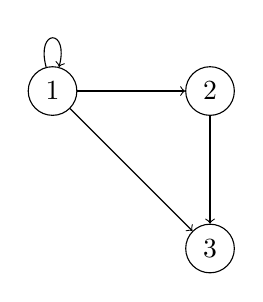
\begin{tikzpicture}[->,node distance=2cm]
  \node[draw,circle] (A) {$1$};
  \node[draw,circle] (B) [right of=A] {$2$};
  \node[draw,circle] (C) [below of=B] {$3$};
  \draw (A) to [loop above]  (A);
  \draw (A) to  (B);
  \draw (A) to  (C);
  \draw (B) to  (C);
  \end{tikzpicture}
\end{align*}
\end{ex}

\begin{prob}
  $\{1,2,3,4\}$ kümesi üzerinde $\le$ ile gösterilen küçük veya eşittir bağıntısını bir
  çizge olarak ele alın ve buna karşılık gelen şemayı çizin.
\end{prob}

\end{document}
